\section{The backend (API)}

\subsection{Module structure}

The API in \texttt{backend/src/} is an Express 5 application in TypeScript, executed with \texttt{tsx}. \autoref{tab:api-modules} lists its modules.

\begin{longtable}{|p{0.20\textwidth}|p{0.72\textwidth}|}
	\hline
	\textbf{Module} & \textbf{Responsibility} \\
	\hline
	\endhead
	\texttt{index.\allowbreak{}ts} & Entry point: creates the HTTP and Socket.IO servers on one port, authenticates WebSocket connections, starts the queue event listener, shuts down cleanly on SIGINT/SIGTERM. \\
	\hline
	\texttt{app.\allowbreak{}ts} & Builds the Express application: CORS, JSON body parser (1\,MB), cookie parser, routers, health endpoint, 404 handler and the central error handler. \\
	\hline
	\texttt{config.\allowbreak{}ts} & Loads \texttt{.\allowbreak{}env}, validates all settings with Zod, exposes a typed \texttt{config} object. \\
	\hline
	\texttt{db.\allowbreak{}ts} & The single shared Prisma client. \\
	\hline
	\texttt{auth.\allowbreak{}ts} & Signing and checking session tokens, cookie options, the \texttt{requireAuth} middleware. \\
	\hline
	\texttt{routes/auth.\allowbreak{}ts} & \texttt{/api/auth/*}: register, log in, log out, current user. \\
	\hline
	\texttt{routes/matches.\allowbreak{}ts} & \texttt{/api/matches/*}: upload, list, get, video streaming, results, re-analyse, cancel, report, delete. \\
	\hline
	\texttt{queue.\allowbreak{}ts} & The BullMQ queue: adding, removing and cancelling jobs, counting workers, and turning queue events into database updates. \\
	\hline
	\texttt{storage.\allowbreak{}ts} & Storage folders, safe resolution of stored paths, file deletion, video signature check. \\
	\hline
	\texttt{report.\allowbreak{}ts} & Builds the statistics for the language model, calls Azure OpenAI and translates its errors. \\
	\hline
	\texttt{colours.\allowbreak{}ts} & Turns a measured kit colour into a plain name for the report. \\
	\hline
	\texttt{matchView.\allowbreak{}ts} & \texttt{toPublicMatch()}: the form of a match sent to browsers, without internal file paths. \\
	\hline
	\caption{Modules of the API}
	\label{tab:api-modules}
\end{longtable}

\subsection{REST API}

All endpoints are under \texttt{/api} and exchange JSON, except uploads and file downloads. Errors always have the form \texttt{\{"error": "message"\}} with a fitting HTTP status. All match endpoints need a valid session cookie.

\begin{longtable}{|p{0.10\textwidth}|p{0.27\textwidth}|p{0.54\textwidth}|}
	\hline
	\textbf{Method} & \textbf{Path} & \textbf{Description and responses} \\
	\hline
	\endhead
	POST & \texttt{/auth/register} & Body \texttt{\{name, email, password\}}. Creates the user and sets the session cookie. 201; 400 invalid input; 409 e-mail exists. \\
	\hline
	POST & \texttt{/auth/login} & Body \texttt{\{email, password\}}. Sets the session cookie. 200 \texttt{\{user\}}; 401 wrong credentials. \\
	\hline
	POST & \texttt{/auth/logout} & Clears the cookie. 204. \\
	\hline
	GET & \texttt{/auth/me} & The logged-in user. 200 \texttt{\{user\}}; 401 not logged in or account deleted. \\
	\hline
	POST & \texttt{/matches} & Multipart form with \texttt{video}, \texttt{title}, \texttt{mode}. Stores the file, creates the match, queues the job. 201 \texttt{\{match\}}; 400 no or invalid file; 413 too large. \\
	\hline
	GET & \texttt{/matches} & The user's matches, newest first. 200 \texttt{\{matches\}}. \\
	\hline
	GET & \texttt{/matches/:id} & One match. 200 \texttt{\{match\}}; 404 not found or not owned. \\
	\hline
	GET & \texttt{/\allowbreak{}matches/\allowbreak{}:id/\allowbreak{}video} & Streams the playback copy (or the original) with HTTP Range support for seeking. 200 or 206. \\
	\hline
	GET & \texttt{/\allowbreak{}matches/\allowbreak{}:id/\allowbreak{}results} & The results file. 200; 409 not finished. \\
	\hline
	POST & \texttt{/\allowbreak{}matches/\allowbreak{}:id/\allowbreak{}reanalyse} & Optional body \texttt{\{mode\}}. Queues the analysis again. 200 \texttt{\{match\}}; 409 already queued or running. \\
	\hline
	POST & \texttt{/\allowbreak{}matches/\allowbreak{}:id/\allowbreak{}cancel} & Stops a queued or running analysis. 200 \texttt{\{match\}} (cancelled, or still processing with stage ``Cancelling\dots''); 409 not being analysed. \\
	\hline
	GET & \texttt{/\allowbreak{}matches/\allowbreak{}:id/\allowbreak{}report} & 200 \texttt{\{report, enabled\}}; \texttt{enabled} says whether reports are configured. \\
	\hline
	POST & \texttt{/\allowbreak{}matches/\allowbreak{}:id/\allowbreak{}report} & Generates and stores the report. 200 \texttt{\{report\}}; 409 not finished; 429, 502 or 503 report service errors. \\
	\hline
	DELETE & \texttt{/matches/:id} & Deletes the match, its waiting job and its files. 204; 409 while processing. \\
	\hline
	GET & \texttt{/health} & Database, Redis, number of workers and job counts. 200 when healthy, 503 otherwise. \\
	\hline
	\caption{REST endpoints}
	\label{tab:endpoints}
\end{longtable}

The WebSocket interface has one event. After connecting, the server puts each socket into a private room \texttt{user:<id>}; whenever one of the user's matches changes, it emits \texttt{match:updated} with the public match to that room only.

\subsection{Important functions}

\begin{longtable}{|p{0.22\textwidth}|p{0.26\textwidth}|p{0.43\textwidth}|}
	\hline
	\textbf{Function} & \textbf{Input $\rightarrow$ output} & \textbf{Activity} \\
	\hline
	\endhead
	\texttt{requireAuth} (auth.ts) & request $\rightarrow$ \texttt{req.\allowbreak{}userId}, or 401 & Reads the \texttt{token} cookie, checks the JWT signature and expiry, attaches the user ID. \\
	\hline
	\texttt{signToken} / \texttt{verifyToken} & user ID $\leftrightarrow$ JWT & HS256-signed token with the user ID as subject, valid for 7 days~\cite{jwt}. \\
	\hline
	\texttt{findOwnMatch} (matches.ts) & request $\rightarrow$ match, or 404 & Loads a match by ID \emph{and} owner; answers 404, not 403, for other users' matches so their IDs cannot be probed. \\
	\hline
	\texttt{isVideoFile} (storage.ts) & file path $\rightarrow$ boolean & Checks the first 12 bytes for the signatures of MP4/MOV, Matroska/WebM and AVI. \\
	\hline
	\texttt{absolutePath} (storage.ts) & relative path $\rightarrow$ absolute path & Refuses any path that would leave the storage folder. \\
	\hline
	\texttt{enqueueAnalysis} (queue.ts) & \texttt{\{matchId, videoPath, mode\}} $\rightarrow$ void & Removes a finished job with the same ID (BullMQ ignores duplicate IDs), deletes any old cancel note, adds the job with the match ID as job ID. \\
	\hline
	\texttt{requestCancel} (queue.ts) & match ID $\rightarrow$ \texttt{"removed"} or \texttt{"stopping"} & Removes a waiting job; if the job is running, writes the cancel note (expires after a day). A missing job counts as removed. \\
	\hline
	\texttt{cancelledState} (queue.ts) & match $\rightarrow$ database fields & \texttt{COMPLETED} with stage ``Re-analysis cancelled'' if the match has earlier results, otherwise \texttt{CANCELLED}. \\
	\hline
	\texttt{countWorkers} (queue.ts) & $\rightarrow$ number & Counts distinct worker connections in Redis's client list, recognising the Node.js and Python naming schemes. \\
	\hline
	\texttt{start\allowbreak{}Queue\allowbreak{}Event\allowbreak{}Listener} & callback $\rightarrow$ listener & Turns \texttt{active}, \texttt{progress}, \texttt{completed} and \texttt{failed} events into database updates and calls the callback with each updated match. \\
	\hline
	\texttt{buildMatchData} (report.ts) & match $\rightarrow$ statistics object & Reads the results file and builds the model's input: summary, kit colour names, formation timeline, shape per third of the video, the three positions that ran furthest. \\
	\hline
	\texttt{colourName} (colours.ts) & hex colour $\rightarrow$ name & HSL rules: white, black, greys, then a hue name with ``dark'' or ``light'' (\autoref{sec:report}). \\
	\hline
	\texttt{generate\allowbreak{}Coaching\allowbreak{}Report} & match $\rightarrow$ Markdown & Builds the statistics, calls the model, maps its errors to \texttt{ReportError} with an HTTP status. \\
	\hline
	\caption{Important functions of the API}
	\label{tab:api-functions}
\end{longtable}

\subsection{Upload handling}

Multer streams an upload to disk while it arrives, so even a 1\,GB video never has to fit in memory. The file gets a random UUID name, and only files with a video extension and a \texttt{video/*} MIME type are accepted. Both are supplied by the client and can be faked, so the API also reads the file's first bytes after the upload and deletes it if they are not those of a video container. Then the match row is created and the job queued. If the queue cannot be reached, the match is kept but marked failed with ``Could not queue the analysis job'', so the user can retry with Re-analyse instead of uploading again.

\subsection{Turning queue events into live updates}

The queue events of one job arrive in bursts, for example several progress events within milliseconds. In the first version each event started its own database update, a slower update sometimes finished after a newer one, and the progress bar jumped backwards. The listener now chains the updates of each match: every update waits for the previous update of the same match, while different matches proceed in parallel (\autoref{code:chain}). The \texttt{failed} event checks whether the job has attempts left; if so, the match goes back to \texttt{QUEUED} with ``Retrying after an error''. The \texttt{completed} event checks for \texttt{\{cancelled: true\}} and then applies \texttt{cancelledState} instead of storing results.

\begin{lstlisting}[language=TypeScript, caption={Per-match ordering of database updates (from \texttt{backend/src/queue.\allowbreak{}ts})}, label={code:chain}]
const chains = new Map<string, Promise<void>>();
const update = (matchId: string, data: MatchUpdate) => {
  const next = (chains.get(matchId) ?? Promise.resolve()).then(async () => {
    // Updates for matches deleted in the meantime are simply dropped.
    const match = await prisma.match.update({ where: { id: matchId }, data }).catch(() => null);
    if (match) onUpdate(match);   // push to the user's browser
  });
  chains.set(matchId, next);
  void next.finally(() => { if (chains.get(matchId) === next) chains.delete(matchId); });
  return next;
};
\end{lstlisting}

\subsection{Cancelling an analysis}
\label{sec:cancel}

The coach who uploads the wrong video, or picks Standard instead of Quick, should not have to wait an hour. A queued job is easy: BullMQ can remove a waiting job. A running job cannot be taken away from the worker that holds its lock, so the API leaves a note in Redis (\texttt{tactical-eye:cancel:<match\allowbreak{}Id>}) and shows ``Cancelling\dots''. The worker checks for the note every two seconds in a background task. When it finds one, it sets a flag, and the next progress report from the analysis thread raises \texttt{Analysis\allowbreak{}Cancelled}, which stops the pipeline wherever it is. The pipeline reports progress hundreds of times per analysis, so this needs no checks in the individual stages. The worker then deletes a half-written playback copy if the match had no earlier results and returns \texttt{\{cancelled: true\}}. When the analysis runs on the GPU, the worker also calls the GPU service's cancel endpoint, so the GPU becomes free for the next job. In the system test the worker stopped 4 seconds after the request.

\subsection{Error handling}

Express 5 forwards errors thrown in asynchronous handlers to the error middleware, so route code can simply throw. The central handler in \texttt{app.\allowbreak{}ts} turns validation errors (Zod) into 400 with a readable description of the invalid fields, upload errors (Multer) into 413 for oversized files and 400 otherwise, and everything else into 500 ``Internal server error'', logging the details on the server without showing them to the client. Expected errors (not found, wrong state) are answered in the routes with 404 or 409.

\subsection{The coaching report}
\label{sec:report}

\texttt{report.\allowbreak{}ts} prepares a compact summary of the match for the model: the stored summary, each team's kit colour, defended goal and formation timeline, the team shape averaged over each third of the video, the three positions that ran furthest, and the formation changes. It is sent with a system prompt that defines the sections and the rules: every statement must rest on the numbers, passes, shots and goals must never be invented, and the conclusions are tentative because the camera does not show every player.

The first reports said ``Team A (kit \#C7C9AA)'' and ``Player \#17'', which no coach can use. Two changes fixed this. \texttt{colourName} turns the measured colour into a plain name with simple HSL rules: very light colours with little saturation are white, colours with almost no chroma are black or a shade of grey, and the rest are named by hue with ``dark'' or ``light'' added by lightness. The rules allow for the camera making kits paler or greyer than they are, and dark blues count as colour much sooner than other hues, because navy kits look grey on video. A test checks the colours measured on the real videos: Real Madrid's \texttt{\#C7C9AA} is ``white'', PSG's \texttt{\#4E525D} ``navy'' and Barcelona's away kit \texttt{\#A27051} ``orange''. The runners are now sent as positions with full names (``LB (left back)''), and the prompt forbids colour codes and player numbers. A test also checks that the data sent to the model contains neither.

The request goes to a \texttt{gpt-5-mini} deployment on Azure OpenAI through the \texttt{AzureOpenAI} client of the official \texttt{openai} SDK, with a 120-second timeout and two automatic retries. The output limit is 8,000 tokens because reasoning models spend tokens on hidden reasoning before writing. I chose Azure OpenAI because its use is covered by the Azure for Students credit, and kept all provider-specific code in this one module.

\section{The AI worker}

\subsection{Modules}

\begin{longtable}{|p{0.22\textwidth}|p{0.70\textwidth}|}
	\hline
	\textbf{Module} & \textbf{Responsibility} \\
	\hline
	\endhead
	\texttt{worker.\allowbreak{}py} & Queue consumer: takes jobs, runs the analysis in a thread, forwards progress, watches for cancel notes, chooses between remote and local analysis, keeps the ``done'' notes. \\
	\hline
	\texttt{src/config.\allowbreak{}py} & Every parameter and threshold in one place, each with a comment explaining its value. \\
	\hline
	\texttt{src/pipeline.\allowbreak{}py} & \texttt{run\_\allowbreak{}analysis()}: runs the stages, reports progress, times each stage, measures memory, builds and writes the results and the summary. \\
	\hline
	\texttt{src/video.\allowbreak{}py}, \texttt{src/transcode.\allowbreak{}py} & Video metadata and batched frame reading; the H.264 playback copy. \\
	\hline
	\texttt{src/detector.\allowbreak{}py} & \texttt{Football\allowbreak{}Detector}: YOLOv8 inference and class mapping. \\
	\hline
	\texttt{src/tracker.\allowbreak{}py} & \texttt{FootballTracker}, \texttt{iter\_\allowbreak{}tracks}: ByteTrack and the tracks table. \\
	\hline
	\texttt{src/homography.\allowbreak{}py} & Pitch landmarks, homography fitting, smoothing and projection. \\
	\hline
	\texttt{src/cleanup.\allowbreak{}py} & Removing people off the pitch, choosing the real ball, joining broken tracks. \\
	\hline
	\texttt{src/clustering.\allowbreak{}py} & Roles, shirt colours, teams, referees, formation templates and detection. \\
	\hline
	\texttt{src/positions.\allowbreak{}py} & Slot names and the position labels. \\
	\hline
	\texttt{src/trajectories.\allowbreak{}py}, \texttt{src/metrics.\allowbreak{}py} & Smoothing and ball interpolation; team shape, statistics, heatmaps. \\
	\hline
	\texttt{src/cancel.\allowbreak{}py} & \texttt{Analysis\allowbreak{}Cancelled} and the name of the cancel note. \\
	\hline
	\texttt{src/remote.\allowbreak{}py}, \texttt{gpu\_\allowbreak{}server.\allowbreak{}py} & Client of the remote GPU service, and the service itself (FastAPI). \\
	\hline
	\caption{Modules of the worker}
	\label{tab:worker-modules}
\end{longtable}

The stage modules do not know about the queue or the web platform. They take and return DataFrames and can be used from scripts and tests. \autoref{fig:classes} shows the main classes.

\begin{figure}[H]
	\centering
	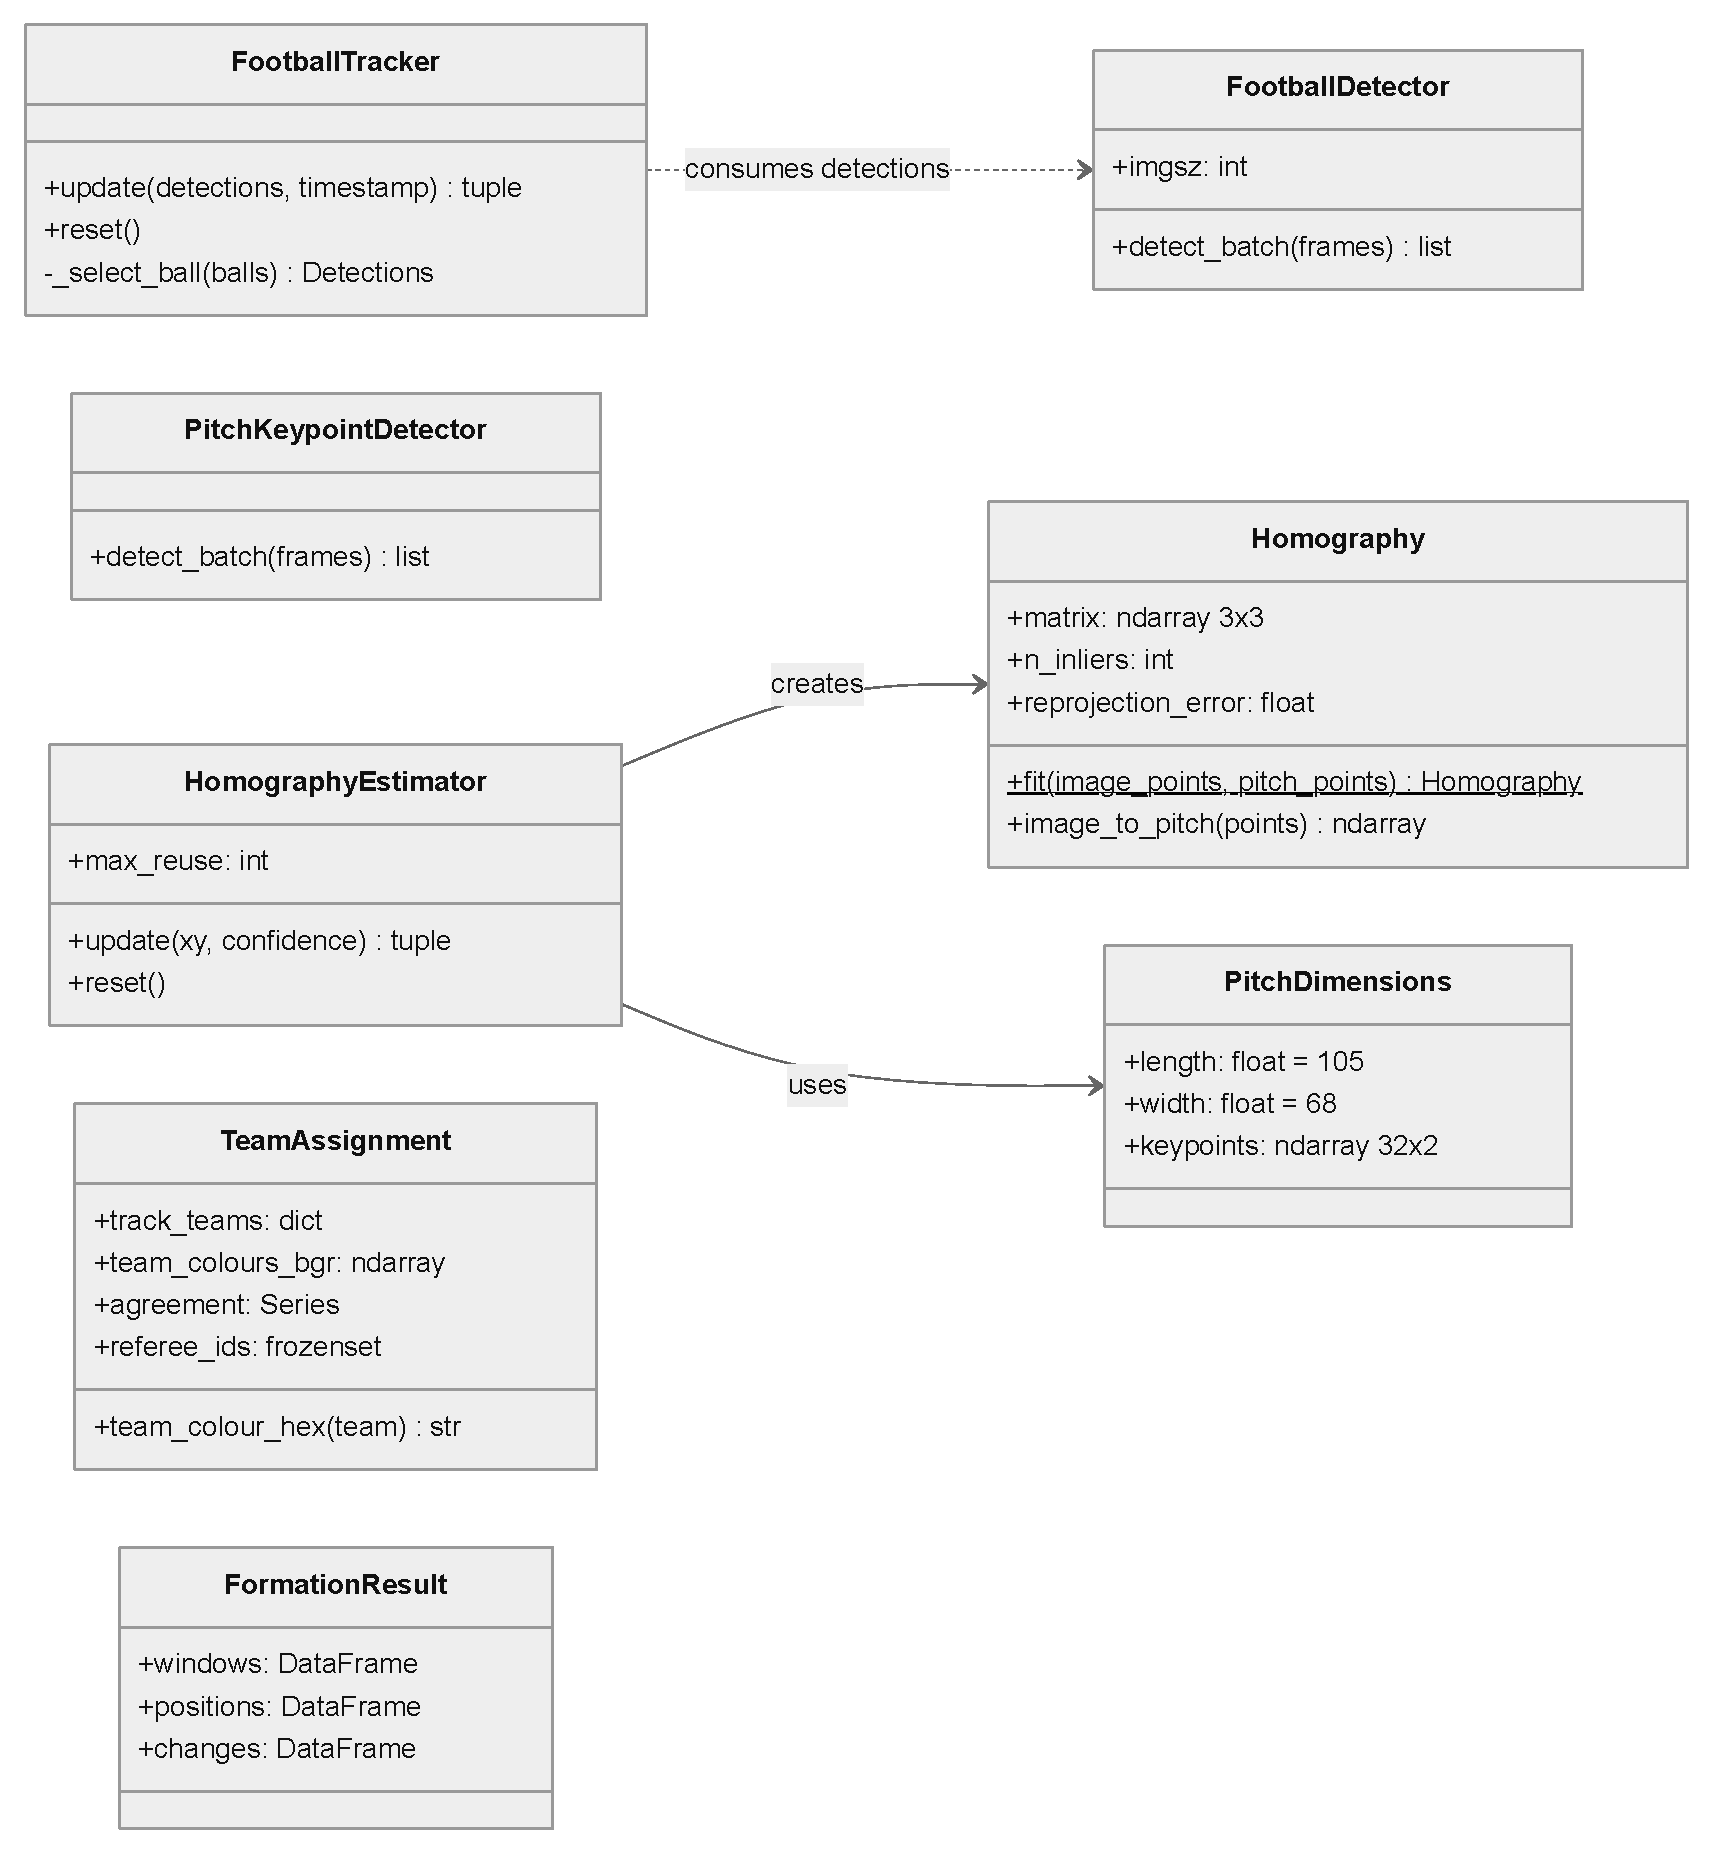
\includegraphics[width=\textwidth]{classes_worker}
	\caption{Main classes of the worker}
	\label{fig:classes}
\end{figure}

\subsection{Important functions}

\autoref{tab:worker-functions} gives the input, output and activity of the worker's key functions, in the order in which the pipeline calls them. ``Tracks'' means the tracks table, one row per detection per analysed frame.

\begin{longtable}{|p{0.22\textwidth}|p{0.30\textwidth}|p{0.39\textwidth}|}
	\hline
	\textbf{Function} & \textbf{Input $\rightarrow$ output} & \textbf{Activity} \\
	\hline
	\endhead
	\texttt{analyse} (worker.py) & queue job $\rightarrow$ \texttt{\{resultPath, playbackPath, summary\}} or \texttt{\{cancelled\}} & Returns a saved result if this run of the job has already finished; otherwise runs the analysis remotely or locally in a thread while watching for cancel notes, and saves a ``done'' note. \\
	\hline
	\texttt{run\_\allowbreak{}analysis} (pipeline.py) & video path, results path, playback path, progress callback, mode $\rightarrow$ summary dict & Runs every stage, measures peak RAM and GPU memory, writes the results file atomically and returns the summary with stage times and file sizes. \\
	\hline
	\texttt{make\_\allowbreak{}web\_\allowbreak{}video} (transcode.py) & source path, target path, frame callback $\rightarrow$ target path & Re-encodes to H.264 at a constant frame rate, one output frame per input frame, with ``faststart''. \\
	\hline
	\texttt{iter\_\allowbreak{}tracks} (tracker.py) & video, detector, stride $\rightarrow$ stream of \texttt{FrameTracks} & Reads frames in batches of four, detects, tracks people with ByteTrack, passes up to five ball candidates. \\
	\hline
	\texttt{iter\_\allowbreak{}homographies} (homography.py) & video, landmark detector, stride $\rightarrow$ stream of homographies & Detects landmarks and fits a RANSAC homography per frame, reusing the last one for up to 10 frames. \\
	\hline
	\texttt{smooth\_\allowbreak{}homographies} (homography.py) & homographies, image size, fps $\rightarrow$ homographies & Smooths the camera model over 1.5\,s via four fixed image points (\autoref{sec:camera-smoothing}). \\
	\hline
	\texttt{project\_\allowbreak{}tracks} (homography.py) & tracks, homographies, frame gap $\rightarrow$ tracks with \texttt{pitch\_\allowbreak{}x}, \texttt{pitch\_\allowbreak{}y} & Joins each row to the nearest homography and projects all foot points at once (\autoref{code:projection}). \\
	\hline
	\texttt{remove\_\allowbreak{}off\_\allowbreak{}pitch\_\allowbreak{}people} (cleanup.py) & tracks $\rightarrow$ tracks & Drops non-referee tracks whose median position is more than 0.5\,m outside the pitch. \\
	\hline
	\texttt{select\_\allowbreak{}ball} (cleanup.py) & tracks with ball candidates $\rightarrow$ tracks with at most one ball per frame & Follows the ball's path (\autoref{alg:ball}). \\
	\hline
	\texttt{extract\_\allowbreak{}jersey\_\allowbreak{}features} (clustering.py) & video, tracks $\rightarrow$ table of Lab colours per sample & Crops up to 10 samples per track in one pass over the video and measures the torso colour against the local grass. \\
	\hline
	\texttt{assign\_\allowbreak{}teams} (clustering.py) & tracks, colour samples $\rightarrow$ \texttt{TeamAssignment} & K-Means into two teams, removes referee-coloured tracks and clusters again, places goalkeepers by position. \\
	\hline
	\texttt{find\_\allowbreak{}referees} (clustering.py) & colour samples, roles, team colours, usual positions $\rightarrow$ set of track IDs & Learns the referee kit from the referee tracks and returns players (and goalkeepers outside both boxes) that wear it (\autoref{eq:referee}). \\
	\hline
	\texttt{add\_\allowbreak{}team\_\allowbreak{}column} (clustering.py) & tracks, assignment $\rightarrow$ tracks with \texttt{team}, \texttt{role} & Adds each row's team and role; relabels the found referees. \\
	\hline
	\texttt{stitch\_\allowbreak{}tracks} (cleanup.py) & tracks $\rightarrow$ tracks with new IDs & Joins broken pieces with the Hungarian algorithm and renumbers from 1. \\
	\hline
	\texttt{smooth\_\allowbreak{}positions} (trajectories.py) & tracks $\rightarrow$ tracks & One-second centred rolling mean per person; raw values kept. \\
	\hline
	\texttt{interpolate\_\allowbreak{}ball} (trajectories.py) & tracks $\rightarrow$ tracks with filled ball rows & Fills ball gaps of up to one second linearly; marks the new rows. \\
	\hline
	\texttt{detect\_\allowbreak{}formations} (clustering.py) & tracks $\rightarrow$ \texttt{FormationResult} & Per team and 5-second window: average positions, template matching, hysteresis and the 20-second stability rule. \\
	\hline
	\texttt{match\_\allowbreak{}formation} (clustering.py) & $(n, 2)$ positions $\rightarrow$ cost per formation & Hungarian assignment of players to the slots of each template (\autoref{code:matching}). \\
	\hline
	\texttt{assign\_\allowbreak{}positions} (positions.py) & tracks, formations $\rightarrow$ label per row & Slots of the main formation per window, smoothed per track, unique per frame; GK and REF for goalkeepers and referees. \\
	\hline
	\texttt{team\_\allowbreak{}shape} (metrics.py) & tracks $\rightarrow$ table per frame and team & Outfield players, hull area, width, depth and centroid. \\
	\hline
	\texttt{player\_\allowbreak{}stats} (metrics.py) & tracks, grouping columns $\rightarrow$ table per group & Distance, time visible, average speed and one-second top speed, per track or per team and position. \\
	\hline
	\texttt{heatmap} (metrics.py) & $x$, $y$ arrays $\rightarrow$ $14 \times 21$ grid of shares & Share of positions in each pitch cell. \\
	\hline
	\texttt{run\_\allowbreak{}remote\_\allowbreak{}analysis} (remote.py) & GPU address, token, video, outputs, callback, mode, stop check $\rightarrow$ summary & Uploads in 50\,MB pieces, starts the job, relays progress, cancels on request, downloads the outputs. \\
	\hline
	\caption{Important functions of the worker}
	\label{tab:worker-functions}
\end{longtable}

\subsection{Job processing}

\texttt{worker.\allowbreak{}py} creates a BullMQ \texttt{Worker} with a concurrency of one. The neural networks already use every CPU core, so two analyses at once would only make both slower. The worker registers under a unique name with host name and process ID, which lets the API's health check count workers, and holds a job lock of 120 seconds. If a worker crashes, its lock expires and BullMQ hands the job out again.

The analysis is slow, synchronous code. Run directly in the asynchronous event loop, it would block the loop, the lock would not be renewed and BullMQ would wrongly consider the job stalled. The worker therefore runs the analysis in a separate thread (\texttt{asyncio.\allowbreak{}to\_\allowbreak{}thread}), and progress callbacks from that thread are handed back to the event loop with \texttt{run\_\allowbreak{}coroutine\_\allowbreak{}threadsafe}. Progress is throttled: an update is only forwarded when the integer percentage or the stage text changes. The results file is written atomically, first to a temporary file that then replaces the target in one rename, so the API can never serve a half-written file. Before writing, any remaining \texttt{NaN} or infinity is replaced with \texttt{null} and counted in the log, so one bad value cannot fail a whole analysis.

\subsection{Surviving a sleeping computer}
\label{sec:sleep}

During the long-video runs, my laptop went to sleep while the second half was being analysed on the GPU. The log showed the worker checking the GPU job 28 times a minute until 04:25, then nothing until 05:33. The GPU finished the job in the meantime, but when the laptop woke up, BullMQ saw that the job's lock had not been renewed for over an hour, treated the job as stalled and handed it out again. The worker downloaded the finished results and then started the whole 48-minute analysis a second time; the database never recorded the first completion.

Making sure the laptop stays awake solved that session, but not the weakness. When an analysis finishes, the worker now saves a small note next to the results (\texttt{results/<matchId>.\allowbreak{}done.\allowbreak{}json}) with a fingerprint of the job run and the summary. The fingerprint is the job ID together with the job's creation time: a job handed out again after a stall keeps both, while a deliberate re-analysis creates a new job with a new creation time. When a job starts and finds a note with its own fingerprint, and the result files exist, the worker returns the saved summary at once instead of analysing again. A unit test hands the same job to the worker twice and checks that the analysis runs once, and that a real re-analysis still runs.

\subsection{The remote GPU service}

The optional GPU service (\texttt{gpu\_\allowbreak{}server.\allowbreak{}py}) is a small FastAPI application that runs the same pipeline on a machine with an NVIDIA GPU. It loads the models once at start-up. Every request must carry the shared secret as a Bearer token, and the service refuses to start with a token shorter than 16 characters. I kept the queue worker on the main server and moved only the computation (\autoref{fig:gpu-sequence}). The GPU service never touches the database, the queue or the storage, so it needs no access to the platform's network, and the main server never has to be reachable from the internet.

\begin{figure}[H]
	\centering
	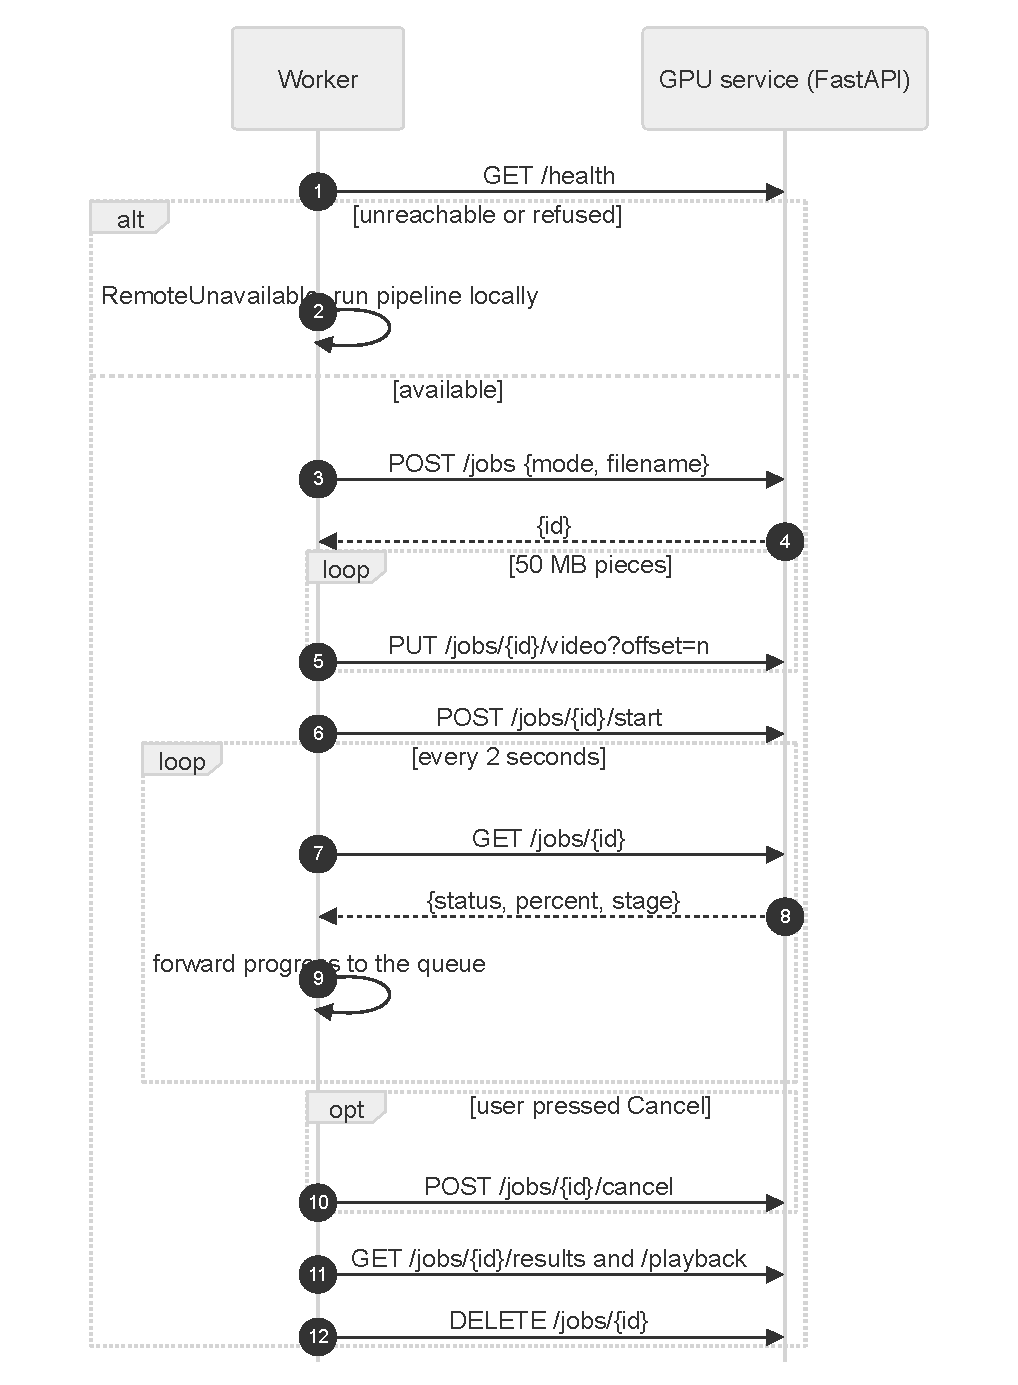
\includegraphics[width=0.75\textwidth]{gpu_sequence}
	\caption{Interaction between the worker and the remote GPU service}
	\label{fig:gpu-sequence}
\end{figure}

The first version uploaded the video in one request, which was fine for 20\,MB clips. A full half is over 500\,MB, and RunPod's HTTP proxy may refuse a request body of that size, so the protocol became three steps: \texttt{POST /jobs} creates an empty job, \texttt{PUT /jobs/\{id\}/video?offset=n} appends one piece of 50\,MB, and \texttt{POST /jobs/\{id\}/start} queues the analysis. Each piece carries its offset, so a piece that is sent twice after a network error is recognised and ignored, and a lost piece is retried up to three times. The 516\,MB first half uploaded in about a minute. The worker also stops waiting after four hours instead of two, enough for a 50\,fps half on a slower GPU.

The client in \texttt{remote.\allowbreak{}py} distinguishes two kinds of failure. \texttt{Remote\allowbreak{}Unavailable} means the service could not be reached or refused the job before any work started; the worker then analyses the video locally. \texttt{Remote\allowbreak{}Analysis\allowbreak{}Error} means the service failed during the job, and the attempt fails as usual and is retried.

\section{The frontend}

\subsection{Structure}

The dashboard in \texttt{frontend/src/} is a single-page application in React 19 and TypeScript, bundled by Vite. Its components form the tree in \autoref{fig:components}, and \autoref{tab:frontend-modules} lists them.

\begin{landscape}
	\begin{figure}
		\centering
		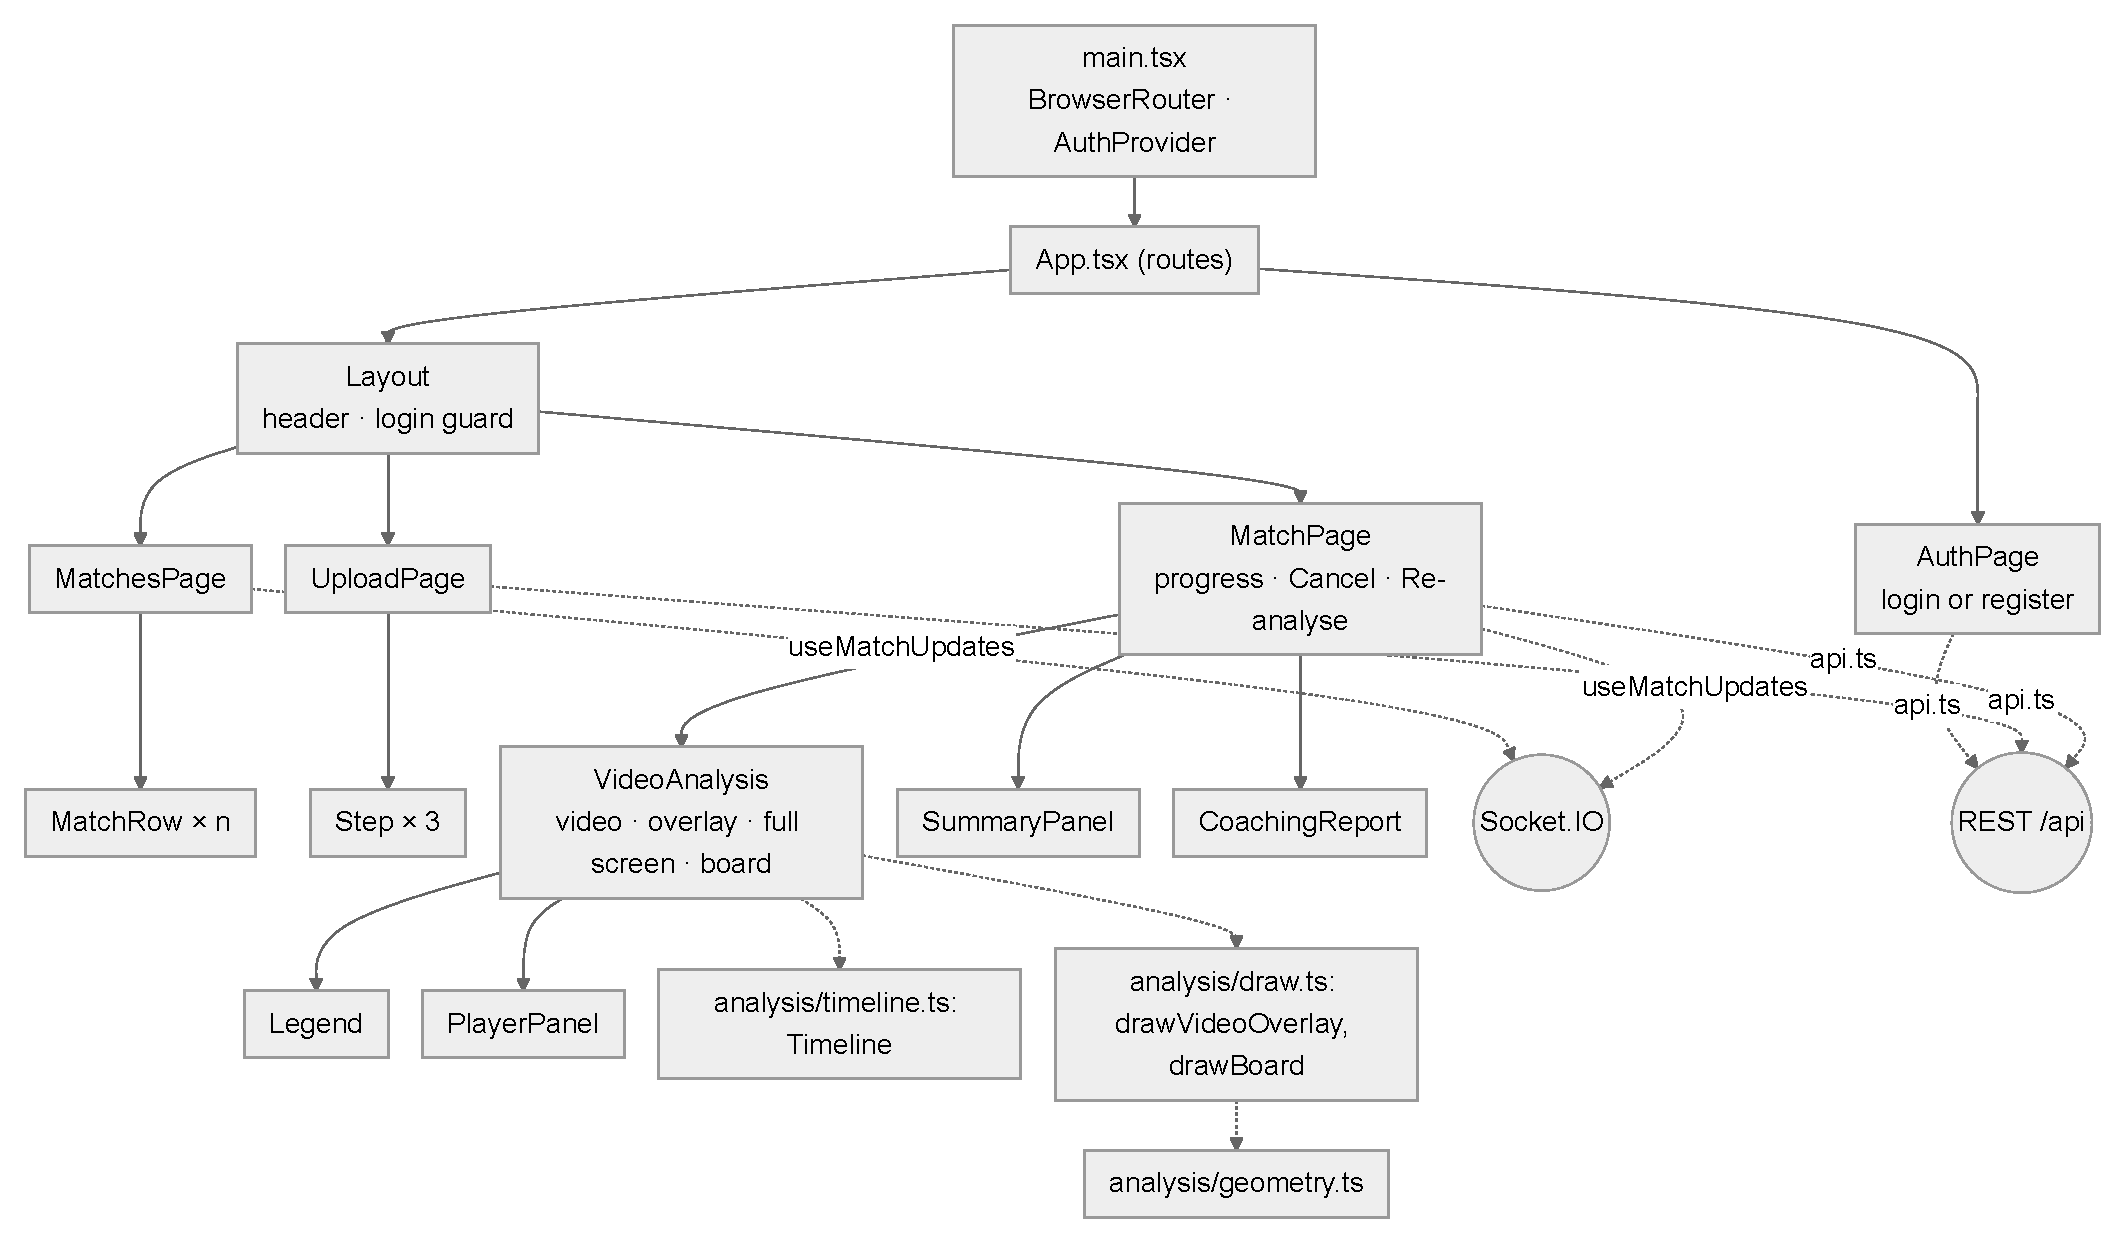
\includegraphics[width=\linewidth,height=0.86\textheight,keepaspectratio]{frontend_components}
		\caption{Component structure of the dashboard}
		\label{fig:components}
	\end{figure}
\end{landscape}

\begin{longtable}{|p{0.24\textwidth}|p{0.68\textwidth}|}
	\hline
	\textbf{Component or module} & \textbf{Responsibility} \\
	\hline
	\endhead
	\texttt{main.\allowbreak{}tsx}, \texttt{App.\allowbreak{}tsx} & Mount the application with the router and the authentication provider; define the routes. \\
	\hline
	\texttt{auth.\allowbreak{}tsx} & \texttt{AuthProvider} and \texttt{useAuth()}: the logged-in user, shared through React context; checks the session with \texttt{/auth/me} on start. \\
	\hline
	\texttt{api.\allowbreak{}ts} & Every REST call; \texttt{ApiError} with message and status; \texttt{uploadMatch()} with upload progress. \\
	\hline
	\texttt{useMatchUpdates.\allowbreak{}ts} & Hook that opens the Socket.IO connection and calls a callback for every \texttt{match:updated} event. \\
	\hline
	\texttt{Layout} & Header and navigation for logged-in pages; sends visitors to the log-in page. \\
	\hline
	\texttt{AuthPage} & Log-in and registration form, one component with two modes. \\
	\hline
	\texttt{MatchesPage}, \texttt{MatchRow} & Match list with live progress and delete confirmation. \\
	\hline
	\texttt{UploadPage}, \texttt{Step} & File by click or drag and drop, title, mode, upload progress. \\
	\hline
	\texttt{MatchPage}, \texttt{SummaryPanel} & Loads the match and its results; progress with Cancel, failure and cancelled notes, the analysis, the summary tab, Re-analyse. \\
	\hline
	\texttt{VideoAnalysis} & Video, overlay canvas, controls, full screen, layer buttons, tactical board, formations, tabs, \texttt{PlayerPanel}. \\
	\hline
	\texttt{CoachingReport} & Loads, generates and renders the Markdown report. \\
	\hline
	\texttt{analysis/timeline.\allowbreak{}ts} & \texttt{Timeline}: where everyone is at any moment, by interpolation; position labels. \\
	\hline
	\texttt{analysis/geometry.\allowbreak{}ts} & Applying and blending homographies, convex hull, fitting a picture into a box. \\
	\hline
	\texttt{analysis/draw.\allowbreak{}ts} & Drawing the video overlay and the board; finding the player under a click. \\
	\hline
	\texttt{components/ui.\allowbreak{}tsx} & Shared elements: button, card, status note, progress bar, error box, spinner, statistic. \\
	\hline
	\caption{Main components and modules of the dashboard}
	\label{tab:frontend-modules}
\end{longtable}

\subsection{Routing and navigation}

\autoref{tab:routes} and \autoref{fig:navigation} show the pages and how the user moves between them. The protected pages are nested inside \texttt{Layout}, which waits for the session check and redirects to \texttt{/login} when nobody is logged in. Unknown addresses redirect to the match list.

\begin{table}[H]
	\centering
	\begin{tabular}{|p{0.2\textwidth}|p{0.24\textwidth}|p{0.47\textwidth}|}
		\hline
		\textbf{Path} & \textbf{Page} & \textbf{Access} \\
		\hline
		\texttt{/login} & \texttt{AuthPage} (log in) & Public; logged-in users are sent to \texttt{/}. \\
		\hline
		\texttt{/register} & \texttt{AuthPage} (register) & Public; logged-in users are sent to \texttt{/}. \\
		\hline
		\texttt{/} & \texttt{MatchesPage} & Logged-in users. \\
		\hline
		\texttt{/upload} & \texttt{UploadPage} & Logged-in users. \\
		\hline
		\texttt{/matches/:id} & \texttt{MatchPage} & The logged-in owner of the match. \\
		\hline
	\end{tabular}
	\caption{Routes of the dashboard}
	\label{tab:routes}
\end{table}

\begin{figure}[H]
	\centering
	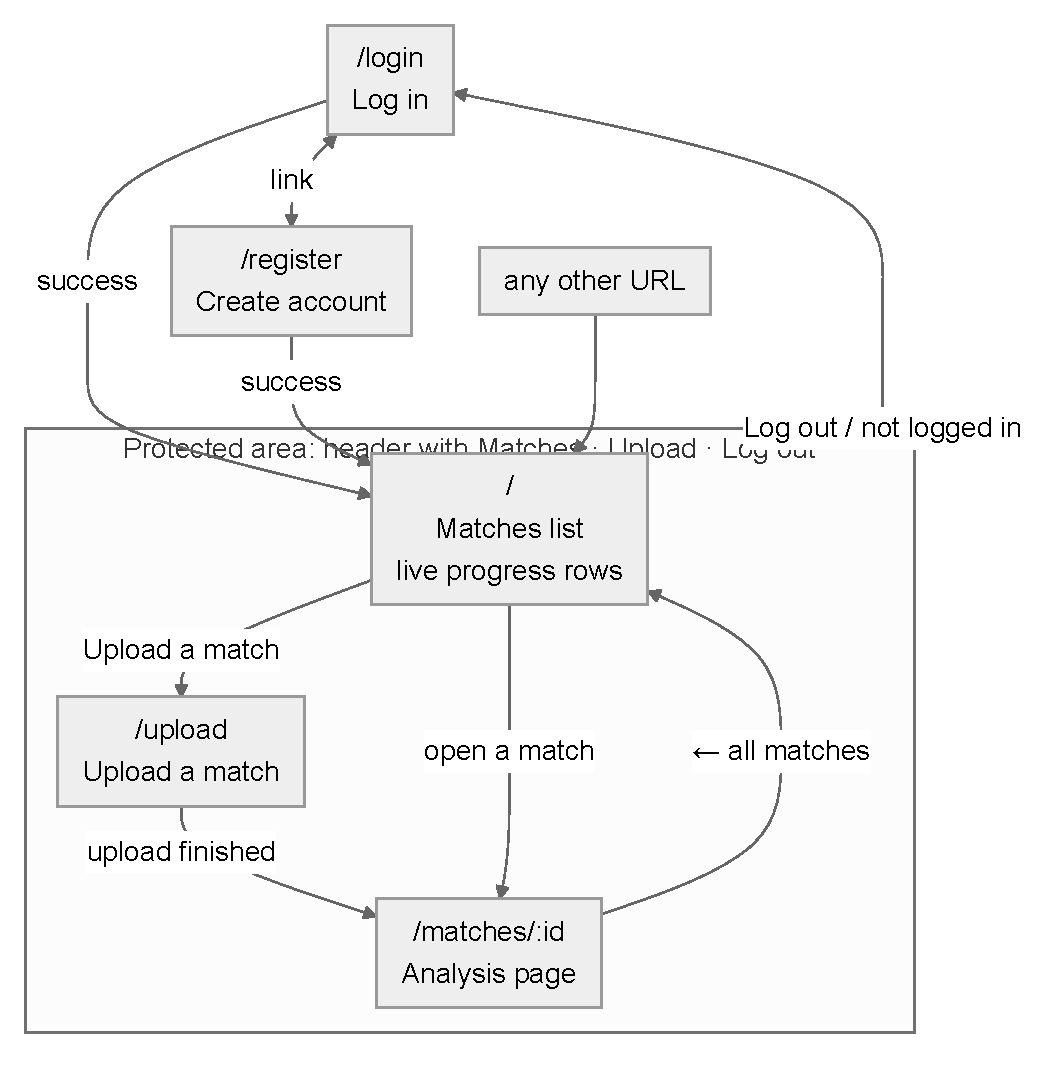
\includegraphics[width=0.75\textwidth]{navigation}
	\caption{Navigation between the pages}
	\label{fig:navigation}
\end{figure}

\subsection{State and live updates}

The dashboard uses React's own state (\texttt{useState}, \texttt{useEffect}) and one context for the logged-in user; no global state library was needed. The session cookie is HTTP-only, so the frontend cannot read it and learns whether the user is logged in from \texttt{/auth/me}. Pages subscribe to live updates with \texttt{use\allowbreak{}Match\allowbreak{}Updates(callback)}. The hook keeps the latest callback in a ref, so the WebSocket opens once per page and does not reconnect on every render. When a match becomes \texttt{COMPLETED}, the match page downloads the results. They are stored together with the completion time they belong to, so after a re-analysis stale results are never combined with new match data.

\subsection{Synchronising the overlays with the video}
\label{sec:overlay-sync}

Keeping the drawings on the players in every frame was the main difficulty of the frontend, and four techniques work together. First, the overlay is redrawn for every displayed frame with \texttt{request\allowbreak{}Video\allowbreak{}Frame\allowbreak{}Callback}~\cite{rvfc}, which reports the exact media time of the frame on screen; the \texttt{timeupdate} event, which I used first, lags up to a quarter of a second behind, and the markers visibly trailed the players. Browsers without the API fall back to \texttt{request\allowbreak{}Animation\allowbreak{}Frame}.

Second, the worker analyses only every 2nd or 4th frame, but the video shows every frame, so \texttt{Timeline.\allowbreak{}stateAt(t)} finds the analysed frames before and after $t$ by binary search and interpolates boxes and pitch positions between them. It never interpolates across a gap longer than three strides, such as a camera cut.

Third, paths and heatmaps are defined on the pitch, but the camera moves. For every frame the results contain the pitch-to-image homography; \texttt{applyHomography} projects pitch points into the current frame (\autoref{code:apply}), and between analysed frames the two matrices are blended. Points behind the camera ($w \le 0$) are skipped. A heatmap therefore appears painted on the grass and stays there while the camera pans, and since the worker smooths the camera model (\autoref{sec:camera-smoothing}), the paths no longer jump when a new camera update arrives.

Fourth, the canvases are redrawn directly in the frame callback, outside React. React state only holds things that change rarely (layer switches, the selection, the displayed time), and the drawing code reads the current switches through refs; re-rendering the component tree 25 to 50 times a second would be far too slow. The canvases are sized to their on-screen size times the device pixel ratio, so the drawings stay sharp, and a \texttt{ResizeObserver} redraws them when the layout changes, which also covers entering full screen.

\begin{lstlisting}[language=TypeScript, caption={Projecting a pitch point into the current video frame (from \texttt{frontend/src/analysis/geometry.\allowbreak{}ts})}, label={code:apply}]
export function applyHomography(h: number[], x: number, y: number): Point | null {
  const w = h[6] * x + h[7] * y + h[8];
  if (w <= 1e-9) return null;          // behind the camera
  return [(h[0] * x + h[1] * y + h[2]) / w, (h[3] * x + h[4] * y + h[5]) / w];
}
\end{lstlisting}

\subsection{The analysis modules}

\autoref{tab:frontend-functions} gives the inputs, outputs and activity of the functions in \texttt{analysis/}, which contain all the overlay logic.

\begin{longtable}{|p{0.24\textwidth}|p{0.30\textwidth}|p{0.37\textwidth}|}
	\hline
	\textbf{Function} & \textbf{Input $\rightarrow$ output} & \textbf{Activity} \\
	\hline
	\endhead
	\texttt{new Timeline} (timeline.ts) & results file $\rightarrow$ timeline & Sorts the frames by time, indexes each frame's people by track ID, remembers whether the file has position labels (version 3). \\
	\hline
	\texttt{Timeline.\allowbreak{}indexAt} & time $\rightarrow$ index of the last analysed frame at or before it, or $-1$ & Binary search over the frame times. \\
	\hline
	\texttt{Timeline.\allowbreak{}stateAt} & time in seconds $\rightarrow$ \texttt{FrameState} (people with box, foot, pitch position, label and selection key; ball; camera matrix) & Interpolates boxes, pitch positions, ball and camera matrix between the neighbouring analysed frames; empty inside long gaps. \\
	\hline
	\texttt{Timeline.\allowbreak{}trail} & track ID, time, seconds $\rightarrow$ pitch points, oldest first & Collects one person's positions over the last seconds (the 4-second movement path). \\
	\hline
	\texttt{Timeline.\allowbreak{}ballTrail} & time, seconds $\rightarrow$ pitch points & The ball's recent positions; stops at the first frame without a ball, so no line crosses the pitch after a gap. \\
	\hline
	\texttt{Timeline.\allowbreak{}fullPath} & position (or track) ID $\rightarrow$ list of path pieces & Every position of a selection over the video, split wherever another player takes over or the player is out of view. \\
	\hline
	\texttt{applyHomography} (geometry.ts) & $3 \times 3$ matrix, $x$, $y$ $\rightarrow$ image point or \texttt{null} & Projects a pitch point into the frame (\autoref{code:apply}); \texttt{null} behind the camera. \\
	\hline
	\texttt{lerpHomography} & two matrices, $\alpha$ $\rightarrow$ matrix & Element-wise blend for moments between analysed frames. \\
	\hline
	\texttt{convexHull} & points $\rightarrow$ hull points & Andrew's monotone chain; used for the team shape. \\
	\hline
	\texttt{fitContain} & source size, box size $\rightarrow$ scale and offset & Where the video sits inside its box, so canvas and video pixels line up. \\
	\hline
	\texttt{draw\allowbreak{}Video\allowbreak{}Overlay} (draw.ts) & canvas, size, results, timeline, frame state, layers, selection $\rightarrow$ drawing & Draws heatmap, team shape, paths, players with labels and the ball onto the video canvas, in this order. \\
	\hline
	\texttt{drawBoard} & canvas, size, results, timeline, frame state, layers, selection, options $\rightarrow$ drawing & Draws the chalk pitch, heatmap, static path, shapes, paths, people and ball on the board; also used for the small pitch of the \emph{Player} tab. \\
	\hline
	\texttt{personAt} & results, frame state, canvas size, click position $\rightarrow$ selection key or \texttt{null} & Finds the person whose box is nearest to a click on the video, within 25 pixels. \\
	\hline
	\texttt{personOnBoard} & the same for the board $\rightarrow$ selection key or \texttt{null} & Finds the person nearest to a click on the board. \\
	\hline
	\caption{Functions of the frontend analysis modules}
	\label{tab:frontend-functions}
\end{longtable}

\subsection{Event handlers}

\begin{longtable}{|p{0.25\textwidth}|p{0.26\textwidth}|p{0.40\textwidth}|}
	\hline
	\textbf{Handler} & \textbf{Input $\rightarrow$ output} & \textbf{Activity} \\
	\hline
	\endhead
	\texttt{AuthPage.\allowbreak{}handleSubmit} & form submit event $\rightarrow$ navigation to \texttt{/}, or error text & Stops the browser's own submit, calls \texttt{login} or \texttt{register}, shows the server's message on failure. \\
	\hline
	\texttt{UploadPage.\allowbreak{}chooseFile} & \texttt{File} $\rightarrow$ chosen file and title & Stores the file, clears old errors, suggests a title from the file name if none is typed. \\
	\hline
	\texttt{UploadPage.\allowbreak{}handleDrop} & drag event $\rightarrow$ chosen file & Stops the browser from opening the file and passes it to \texttt{chooseFile}. \\
	\hline
	\texttt{UploadPage.\allowbreak{}handleSubmit} & form submit event $\rightarrow$ navigation to the new match, or error text & Uploads with progress (\texttt{uploadMatch}), then opens the match page. \\
	\hline
	\texttt{MatchRow.\allowbreak{}handleDelete} & click on \emph{Yes} $\rightarrow$ row removed, or error text & Deletes the match through the API and removes it from the list. \\
	\hline
	\texttt{MatchPage.\allowbreak{}reanalyse} & click $\rightarrow$ updated match (queued) & Queues the analysis again and shows the returned match. \\
	\hline
	\texttt{MatchPage.\allowbreak{}cancel} & click $\rightarrow$ updated match (cancelled or cancelling) & Asks for confirmation, calls \texttt{/cancel} and shows the returned match. \\
	\hline
	\texttt{useMatchUpdates} callback & pushed match $\rightarrow$ new page state & Replaces the match on the page, or in the list, or adds a new one. \\
	\hline
	\texttt{VideoAnalysis.\allowbreak{}onOverlayClick} & mouse event on the video $\rightarrow$ selection changed, or play/pause & Finds the person under the click (\texttt{personAt}); an empty spot toggles playback. \\
	\hline
	\texttt{VideoAnalysis.\allowbreak{}onBoardClick} & mouse event on the board $\rightarrow$ selection changed & The same on the board (\texttt{personOnBoard}). \\
	\hline
	\texttt{VideoAnalysis.\allowbreak{}toggleSelection} & selection key or \texttt{null} $\rightarrow$ new selection, \emph{Player} tab & Selects a position, or clears the selection if it is already selected. \\
	\hline
	\texttt{VideoAnalysis.\allowbreak{}stepFrame} & $-1$ or $+1$ $\rightarrow$ video one frame back or forward & Pauses and seeks to the next frame, aiming slightly inside it so rounding cannot land on its neighbour. \\
	\hline
	\texttt{VideoAnalysis.\allowbreak{}togglePlay} & click $\rightarrow$ playing or paused & Starts or pauses the video. \\
	\hline
	\texttt{VideoAnalysis.\allowbreak{}toggleFullscreen} & click $\rightarrow$ full screen on or off & Puts the player block (video, drawings, controls) into full screen, or leaves it. \\
	\hline
	\texttt{fullscreenchange} listener & browser event $\rightarrow$ \texttt{fullscreen} state & Keeps the button and the layout right when the user leaves full screen with Esc. \\
	\hline
	Frame callback (\texttt{request\allowbreak{}Video\allowbreak{}Frame\allowbreak{}Callback}) & displayed frame's media time $\rightarrow$ redrawn canvases & Computes \texttt{stateAt} for that time and redraws the overlay and the board. \\
	\hline
	\texttt{CoachingReport.\allowbreak{}generate} & click $\rightarrow$ report text, or error text & Requests a new report, shows a spinner meanwhile, then the Markdown or the error. \\
	\hline
	\caption{Important event handlers of the dashboard}
	\label{tab:handlers}
\end{longtable}

\subsection{User interface design}

The first version of the dashboard used rounded cards, an emerald accent and a dark gradient, the default look of many generated interfaces, and my supervisor's feedback was that it looked like one. I redesigned it around the idea of a coach's tactics board: a dark pitch-green background with faint mowing stripes, chalk-white text and dashed lines, an amber accent, IBM Plex fonts, and handwritten Kalam notes for statuses and hints (``ready \checkmark'', ``Drop a video here''). The match list became rows instead of a grid of cards, the upload page a numbered three-step form, and the summary a side-by-side comparison table. On the tactical board, Team A is drawn as circles and Team B as crosses, as on a chalkboard, while the video overlay keeps the real kit colours so that the drawing matches the shirts. Interactive elements have accessible labels, destructive actions need a confirmation, and every asynchronous action shows its state and disables its button against double submission.
